\section{Answers}
%TCIMACRO{\TeXButton{Start Two Columns}{\columnsep =30pt
% \begin {multicols}{2}}}%
%BeginExpansion
\columnsep =30pt
\begin {multicols}{2}
%EndExpansion
 

\textbf{Exercises 3.1} 

1. $\frac{\pi }{5} \approx 0.628 \mbox{rad}$ 

3. $\frac{ -8 \pi }{3} \approx  -8.378 \mbox{rad}$ 

5. $\frac{\pi }{3} \approx 1.047 \mbox{rad}$ 

7. $\frac{ -3 \pi }{4} \approx  -2.356 \mbox{rad}$ 

9. $135 \mbox{{\ensuremath{{}^\circ}}}$ 

11. $150 \mbox{{\ensuremath{{}^\circ}}}$ 

13. $\frac{ -270}{\pi } \approx  -85.9 \mbox{{\ensuremath{{}^\circ}}}$ 

15. $ -15 \mbox{{\ensuremath{{}^\circ}}}$ 

41. $\frac{55 \pi }{9} \approx 19.2$ 

43. $4$ 

45. $4 \mbox{mi}$ 

47. $2 \mbox{rad} \approx 114.6 \mbox{{\ensuremath{{}^\circ}}}$ 

49. $\frac{36}{\pi } \approx 11.459 \mbox{m}$ 

51. $330 \pi  \approx 1037 \mbox{mi}$ 

53. $1.6$ million $\mbox{mi}$ 

55. $1.15 \mbox{mi}$ 

57. $50 \mathrm{m}^{2}$ 

59. $4 \mbox{m}$ 

61. $6 cm^{2}$ 

63. $\frac{32 \pi }{15} ft/\mbox{s}$ 

65.(a) $2000 \pi  rad/\mbox{min}$ (b) $\frac{50 \pi }{3} ft/\mbox{s} \approx 52.4 ft/\mbox{s}$ 

67. $39.3 mi/\mbox{h}$ 

69. $2.1 \mathrm{m}/\mbox{s}$ 

\textbf{Exercises 3.2} 

1. $\sin  \theta  =\frac{4}{5} ,\cos  \theta  =\frac{3}{5} ,\tan  \theta  =\frac{4}{3}$ 

3. $\sin  \theta  =\frac{40}{41} ,\cos  \theta  =\frac{9}{41} ,\tan  \theta  =\frac{40}{9}$ 

5. $\sin  \theta  =\frac{2 \sqrt{13}}{13} ,\cos  \theta  =\frac{3 \sqrt{13}}{13} ,\tan  \theta  =\frac{2}{3}$ 

10. $12 \sqrt{2}$ 

11. $\frac{13 \sqrt{3}}{2}$ 

13. $16.51658$ 

29. $45 \mbox{{\ensuremath{{}^\circ}}} ,16 ,16 \sqrt{2} \approx 22.63$ 

31. $38 \mbox{{\ensuremath{{}^\circ}}} ,44.79 ,56.85$ 

35. $1026 \mbox{ft}$ 

37.(a) $2100 \mbox{mi}$ (b) No 

39. $19 \mbox{ft}$ 

42. $600 \sin  65 \mbox{{\ensuremath{{}^\circ}}} \approx 544 \mbox{ft}$ 

43. $345 \mbox{ft}$ 

45. $415 \mbox{ft} ,152 \mbox{ft}$ 

46.$11,379 \mbox{ft}$ 

49. $5808 \mbox{ft}$ 

\textbf{Exercises 3.3} 

7. $\frac{1}{2}$ 

9. $ -\frac{\sqrt{2}}{2}$ 

11. $ -\sqrt{3}$ 

15. $ -\frac{\sqrt{3}}{2}$ 

17. $\frac{\sqrt{3}}{3}$ 

19. $\frac{\sqrt{3}}{2}$ 

21. $ -1$ 

23. $\frac{1}{2}$ 

29. undefined 

41. $\cos  \theta  = -\frac{4}{5} ,\tan  \theta  = -\frac{3}{4}$ 

43. $\sin  \theta  = -\frac{3}{5} ,\cos  \theta  =\frac{4}{5}$ 

49. (a) $\frac{\sqrt{3}}{2} ,\sqrt{3}$ (b) $\frac{1}{2} ,\frac{\sqrt{3}}{4}$ (c) $\frac{3}{4} ,0.88967$ 

51. $19.1$ 

53. $66.1 \mbox{{\ensuremath{{}^\circ}}}$ 

\textbf{Exercises 3.4} 

1. $318.8$ 

5. $44 \mbox{{\ensuremath{{}^\circ}}}$ 

7. $\angle C =114 \mbox{{\ensuremath{{}^\circ}}} ,a \approx 51 ,b \approx 24$ 

9. $\angle C =62 \mbox{{\ensuremath{{}^\circ}}} ,a \approx 200 b \approx 242$ 
%TCIMACRO{\TeXButton{End Two Columns}{\end {multicols}}}%
%BeginExpansion

%EndExpansion
  

13. $\angle A =100 \mbox{{\ensuremath{{}^\circ}}} ,a \approx 89 ,c \approx 71$ 

15. $\angle B \approx 30 \mbox{{\ensuremath{{}^\circ}}} ,\angle C \approx 40 \mbox{{\ensuremath{{}^\circ}}} ,c \approx 19$ 

17. no solution 

19. $\angle A_{1} \approx 125 \mbox{{\ensuremath{{}^\circ}}} ,\angle C_{1} \approx 30 \mbox{{\ensuremath{{}^\circ}}} ,a_{1} \approx 49\text{,}$ 

\  \ $\angle A_{2} \approx 5 \mbox{{\ensuremath{{}^\circ}}} ,\angle C_{2} \approx 150 \mbox{{\ensuremath{{}^\circ}}} ,a_{2} \approx 5.6$ 

23. $219 \mbox{ft}$ 

25. (b) $1018 \mbox{mi}\text{,}$ (c) $1017 \mbox{mi}$ 

27. $155 \mbox{m}$ 

31. $48.2 \mbox{{\ensuremath{{}^\circ}}}$ 

\textbf{Exercises 3.5} 

1. $28.9$ 

5. $29.89 \mbox{{\ensuremath{{}^\circ}}}$ 

9. $\angle A \approx 39.4 \mbox{{\ensuremath{{}^\circ}}} ,\angle B \approx 20.6 \mbox{{\ensuremath{{}^\circ}}} ,c \approx 24.6$ 

13. $\angle A \approx 50 \mbox{{\ensuremath{{}^\circ}}} ,\angle B \approx 73 \mbox{{\ensuremath{{}^\circ}}} ,\angle C \approx 57 \mbox{{\ensuremath{{}^\circ}}}$ 

15. $\angle A_{1} \approx 83.6 \mbox{{\ensuremath{{}^\circ}}} ,\angle C_{1} \approx 56.4 \mbox{{\ensuremath{{}^\circ}}} ,a_{1} \approx 193$ 

\  \ $\angle A_{2} \approx 16.4 \mbox{{\ensuremath{{}^\circ}}} ,\angle C_{2} \approx 123.6 \mbox{{\ensuremath{{}^\circ}}} ,a_{2} \approx 54.9$ 

19. $2$ 

23. $84.6 \mbox{{\ensuremath{{}^\circ}}}$ 

27. $2.30 \mbox{mi}$ 

29. $23.1 \mbox{mi}$ 

31 $2179 \mbox{mi}$ 

33. (a) $62.6 \mbox{mi}$ (b) $S 18.2 \mbox{{\ensuremath{{}^\circ}}} E$ 

35. $96 \mbox{{\ensuremath{{}^\circ}}}$ 

37. $211 \mbox{ft}$ 

39. $3835 \mbox{ft}$ 

41. $3.85 cm^{2}$ 

43. $14.3 \mbox{m}$ 

45. $ \$165,554$ 

\end {multicols}

%------------------------------------------------------------
%------------------------------------------------------------
%END FIRST HALF ANSWERS
%------------------------------------------------------------
%------------------------------------------------------------

\section{Answers}
\textbf{Exercises} 

\begin {multicols}{2}

5. $P \left (\frac{4}{5} ,\frac{3}{5}\right )$ 

7. $P \left (\frac{ -\sqrt{5}}{3} ,\frac{2}{3}\right )$ 

9. $P \left (\frac{ -\sqrt{2}}{3} ,\frac{ -\sqrt{7}}{3}\right )$ 

13. $\left (0 ,1\right )$ 

15. $\left (\frac{ -\sqrt{3}}{2} ,\frac{1}{2}\right )$ 

17. $\left (\frac{1}{2} ,\frac{ -\sqrt{3}}{2}\right )$ 

19. $\left ( -\frac{1}{2} ,\frac{\sqrt{3}}{2}\right )$ 

21. $\left (\frac{ -\sqrt{2}}{2} ,\frac{ -\sqrt{2}}{2}\right )$ 

23. (a) $\left ( -\frac{3}{5} ,\frac{4}{5}\right )$, (b) $\left (\frac{3}{5} , -\frac{4}{5}\right )$ (c) $\left ( -\frac{3}{5} , -\frac{4}{5}\right )$  \\\relax (d)
$\left ( -\frac{3}{5} , -\frac{4}{5}\right )$ 

\end{multicols}

\textbf{Exercises} 
\begin{multicols}{2}

3.
(a) $\frac{ -\sqrt{3}}{2}$ (b) $\frac{1}{2}$ 

5. (a) $ -1$ (b) $ -1$ 

7. (a) $1$ (b) $ -1$ 

9. (a) $0$ (b) $0$ 

13. (a) $\frac{1}{2}$ (b) $\frac{1}{2}$ 

15. (a) $\frac{\sqrt{3}}{3}$ (b) $\frac{ -\sqrt{3}}{3}$ 

27. $\frac{4}{5} ,\frac{3}{5} ,\frac{4}{3}$ 

29. $\frac{ -\sqrt{11}}{4} ,\frac{\sqrt{5}}{4} ,\frac{ -\sqrt{55}}{5}$ 

35. $0.84147$ 

37. $0.93204$ 

39. $1.02964$ 

41. $ -0.57482\vspace{+5.000000cm}$ 
\end{multicols}
\clearpage

\textbf{Exercises} 
\begin{multicols}{2}

\begin{tabular}[c]{ll}1.  &
	\setlength\fboxrule{0.01in}\setlength\fboxsep{0.2in}\fcolorbox[HTML]{000000}{FFFFFF}{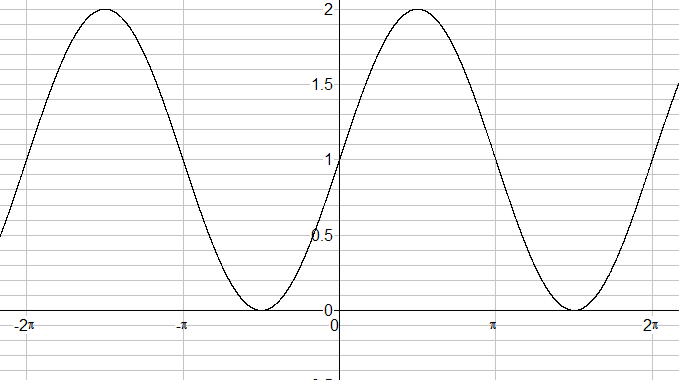
\includegraphics[ width=1.7115in, height=0.9625in,]{L4SZ270N}
	}
	\vspace{0.5cm}  \\
	3.  &
	\setlength\fboxrule{0.01in}\setlength\fboxsep{0.2in}\fcolorbox[HTML]{000000}{FFFFFF}{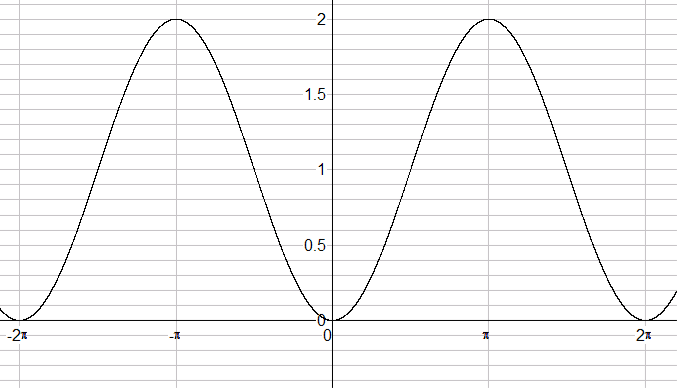
\includegraphics[ width=1.7279in, height=0.9945in,]{L4SZ270O}
	}
	\vspace{0.5cm}  \\
	5.  &
	\setlength\fboxrule{0.01in}\setlength\fboxsep{0.2in}\fcolorbox[HTML]{000000}{FFFFFF}{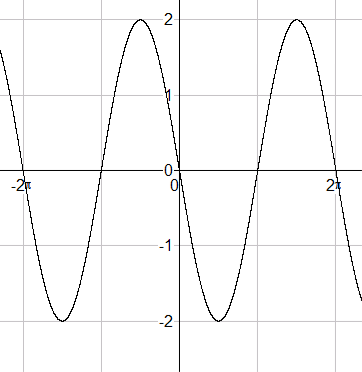
\includegraphics[ width=1.7253in, height=1.7737in,]{L4SZ270P}
	}
	\vspace{0.5cm}  \\
	7.  &
	\setlength\fboxrule{0.01in}\setlength\fboxsep{0.2in}\fcolorbox[HTML]{000000}{FFFFFF}{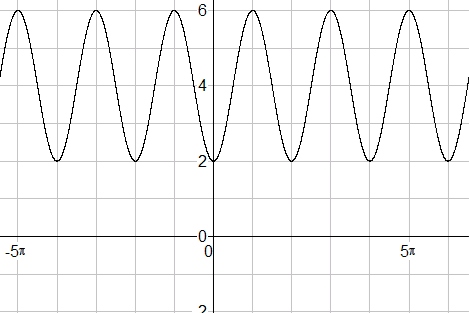
\includegraphics[ width=1.753in, height=1.1727in,]{L4SZ270Q}
	}
	\vspace{0.5cm}  \\
	9.  &
	\setlength\fboxrule{0.01in}\setlength\fboxsep{0.2in}\fcolorbox[HTML]{000000}{FFFFFF}{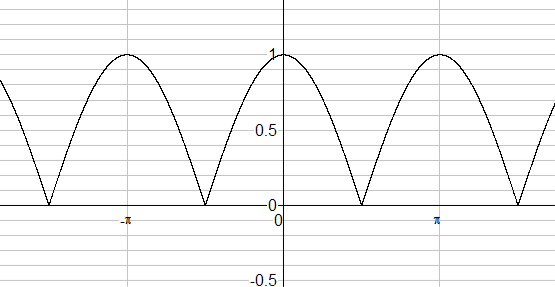
\includegraphics[ width=1.7642in, height=0.9167in,]{L4SZ270R}
	}
	\vspace{0.5cm}
\end{tabular}


\begin{tabular}[c]{ll}11.  & $1 ,\frac{\pi }{2}$  \\
	&    
	\setlength\fboxrule{0.01in}\setlength\fboxsep{0.2in}\fcolorbox[HTML]{000000}{FFFFFF}{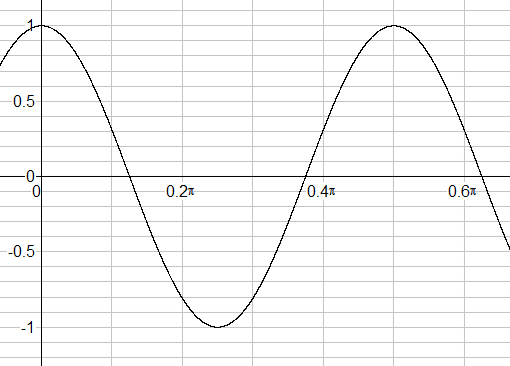
\includegraphics[ width=1.9666in, height=1.4157in,]{L4SZ270S}
	}
\end{tabular}


\begin{tabular}[c]{ll}13.  & $3 ,\frac{2 \pi }{3}$  \\
	&    
	\setlength\fboxrule{0.01in}\setlength\fboxsep{0.2in}\fcolorbox[HTML]{000000}{FFFFFF}{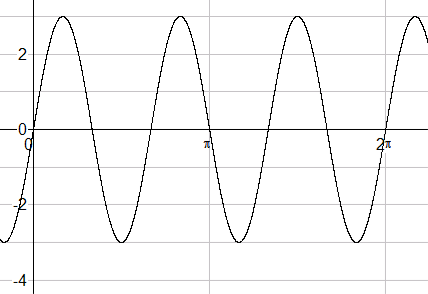
\includegraphics[ width=1.9692in, height=1.3569in,]{L4SZ270T}
	}
\end{tabular}


\begin{tabular}[c]{ll}15.  & $10 ,4 \pi $  \\
	&    
	\setlength\fboxrule{0.01in}\setlength\fboxsep{0.2in}\fcolorbox[HTML]{000000}{FFFFFF}{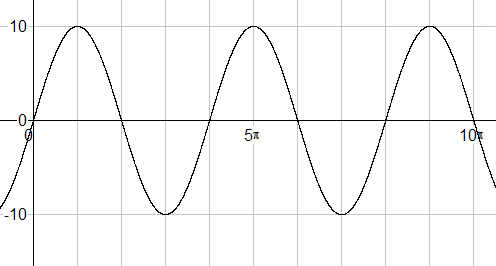
\includegraphics[ width=2.1802in, height=1.1744in,]{L4SZ270U}
	}
\end{tabular}


\begin{tabular}[c]{ll}17.  & $1 ,6 \pi $  \\
	&    
	\setlength\fboxrule{0.01in}\setlength\fboxsep{0.2in}\fcolorbox[HTML]{000000}{FFFFFF}{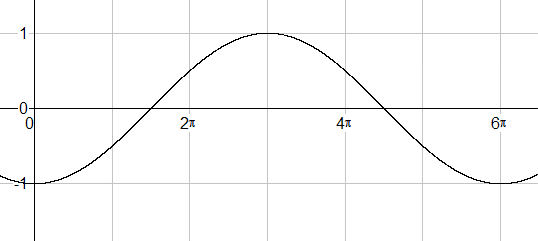
\includegraphics[ width=2.3013in, height=1.036in,]{L4SZ270V}
	}
\end{tabular}


\begin{tabular}[c]{ll}19.  & $3 ,\frac{2}{3}$ note the non-trig scale  \\
	&
	\setlength\fboxrule{0.01in}\setlength\fboxsep{0.2in}\fcolorbox[HTML]{000000}{FFFFFF}{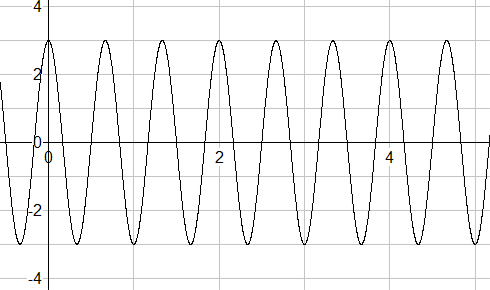
\includegraphics[ width=2.4933in, height=1.4806in,]{L4SZ270W}
	}
\end{tabular}


\begin{tabular}[c]{ll}21.  & $1 ,2 \pi  ,\frac{\pi }{2}$  \\
	&    
	\setlength\fboxrule{0.01in}\setlength\fboxsep{0.2in}\fcolorbox[HTML]{000000}{FFFFFF}{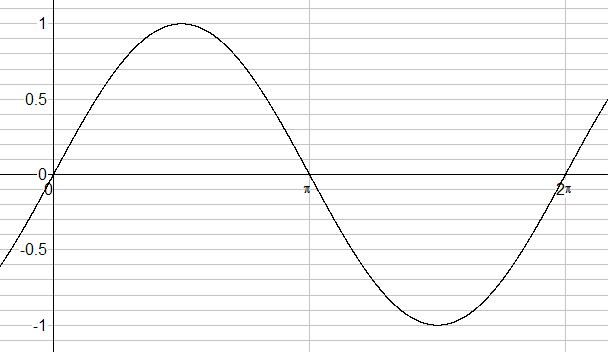
\includegraphics[ width=2.4794in, height=1.4416in,]{L4SZ270X}
	}
\end{tabular}


\begin{tabular}[c]{ll}23.  & $2 ,2 \pi  ,\frac{\pi }{6}$  \\
	&    
	\setlength\fboxrule{0.01in}\setlength\fboxsep{0.2in}\fcolorbox[HTML]{000000}{FFFFFF}{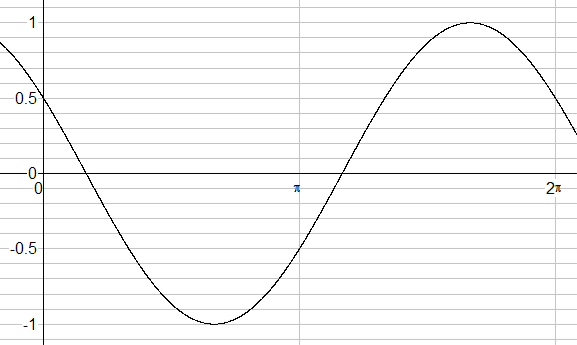
\includegraphics[ width=2.4794in, height=1.4883in,]{L4SZ270Y}
	}
\end{tabular}


\begin{tabular}[c]{ll}25.  & $5 ,\frac{2 \pi }{3} ,\frac{\pi }{12}$  \\
	&    
	\setlength\fboxrule{0.01in}\setlength\fboxsep{0.2in}\fcolorbox[HTML]{000000}{FFFFFF}{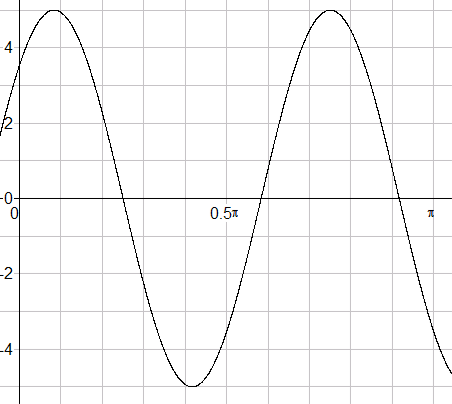
\includegraphics[ width=2.1724in, height=1.9441in,]{L4SZ270Z}
	}
\end{tabular}


\begin{tabular}[c]{ll}27.  & $2 ,3 \pi  ,\frac{\pi }{4}$  \\
	&    
	\setlength\fboxrule{0.01in}\setlength\fboxsep{0.2in}\fcolorbox[HTML]{000000}{FFFFFF}{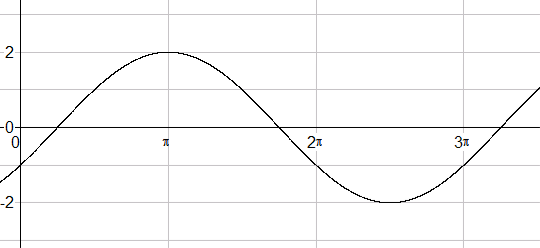
\includegraphics[ width=2.4336in, height=1.1243in,]{L4SZ2710}
	}
\end{tabular}


\begin{tabular}[c]{ll}29.  & $3 ,2 , -\frac{1}{2}$  \\
	&    
	\setlength\fboxrule{0.01in}\setlength\fboxsep{0.2in}\fcolorbox[HTML]{000000}{FFFFFF}{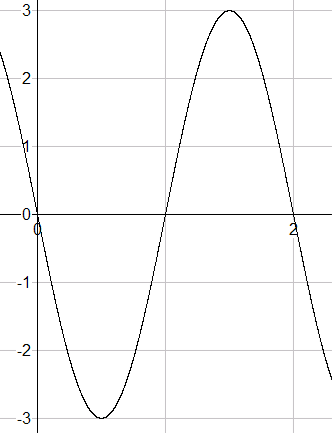
\includegraphics[ width=2.1543in, height=1.8498in,]{L4SZ2711}
	}
\end{tabular}


\begin{tabular}[c]{ll}31.  & $\frac{1}{2} ,\pi  ,\frac{\pi }{6}$  \\
	&    
	\setlength\fboxrule{0.01in}\setlength\fboxsep{0.2in}\fcolorbox[HTML]{000000}{FFFFFF}{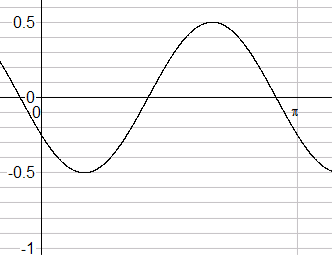
\includegraphics[ width=1.9216in, height=1.4797in,]{L4SZ2712}
	}
\end{tabular}


\begin{tabular}[c]{ll}33.  & $1 ,\frac{2 \pi }{3} , -\frac{\pi }{3}$  \\
	&    
	\setlength\fboxrule{0.01in}\setlength\fboxsep{0.2in}\fcolorbox[HTML]{000000}{FFFFFF}{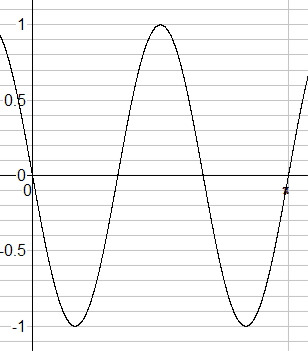
\includegraphics[ width=1.4408in, height=1.6397in,]{L4SZ2713}
	}
\end{tabular}


\begin{tabular}[c]{ll}41.  &  \\
	&
	\setlength\fboxrule{0.01in}\setlength\fboxsep{0.2in}\fcolorbox[HTML]{000000}{FFFFFF}{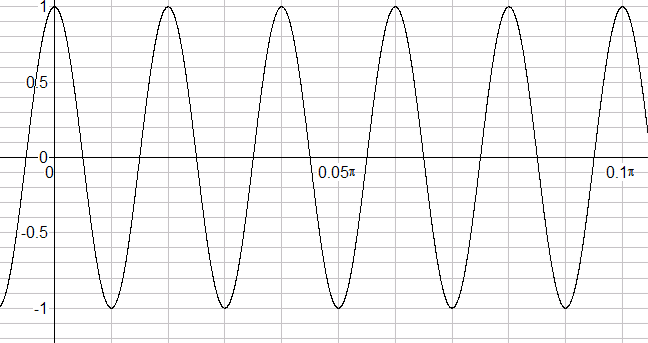
\includegraphics[ width=2.3168in, height=1.2315in,]{L4SZ2714}
	}
\end{tabular}


\begin{tabular}[c]{ll}43.  &  \\
	&
	\setlength\fboxrule{0.01in}\setlength\fboxsep{0.2in}\fcolorbox[HTML]{000000}{FFFFFF}{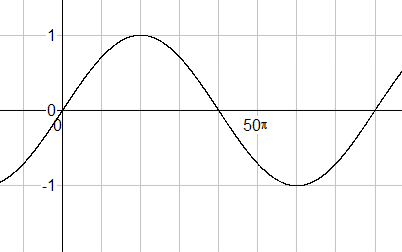
\includegraphics[ width=2.0989in, height=1.3214in,]{L4SZ2715}
	}
\end{tabular}


\begin{tabular}[c]{ll}47.  &  \\
	&
	\setlength\fboxrule{0.01in}\setlength\fboxsep{0.2in}\fcolorbox[HTML]{000000}{FFFFFF}{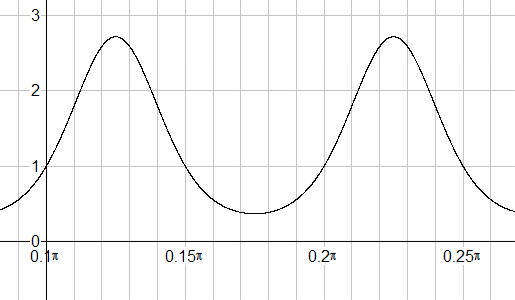
\includegraphics[ width=2.3722in, height=1.3872in,]{L4SZ2816}
	}
\end{tabular}


\begin{tabular}[c]{ll}53.  &  \\
	&
	\setlength\fboxrule{0.01in}\setlength\fboxsep{0.2in}\fcolorbox[HTML]{000000}{FFFFFF}{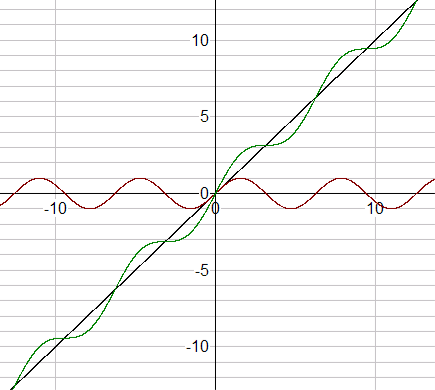
\includegraphics[ width=2.4621in, height=2.2096in,]{L4SZ2817}
	}
\end{tabular}


\begin{tabular}[c]{ll}55.  &  \\
	&
	\setlength\fboxrule{0.01in}\setlength\fboxsep{0.2in}\fcolorbox[HTML]{000000}{FFFFFF}{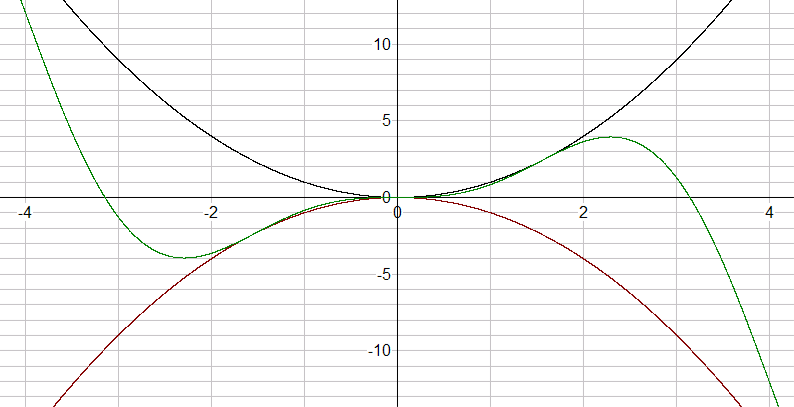
\includegraphics[ width=2.5399in, height=1.3085in,]{L4SZ2818}
	}
\end{tabular}


\begin{tabular}[c]{ll}57.  &  \\
	&
	\setlength\fboxrule{0.01in}\setlength\fboxsep{0.2in}\fcolorbox[HTML]{000000}{FFFFFF}{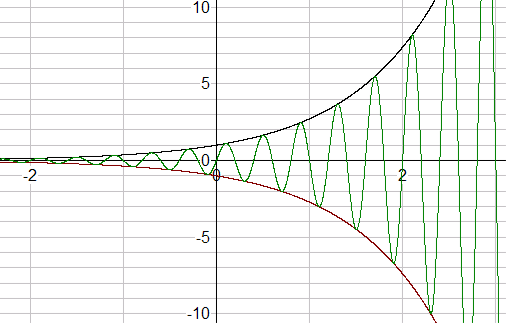
\includegraphics[ width=2.5564in, height=1.6371in,]{L4SZ2819}
	}
\end{tabular}
\end{multicols}

61. Maximum value $1.76$ when $x \approx 0.94$, minimum value $ -1.76$ when $x \approx  -0.94\text{.}$ The same maximum and minimum values occur at infinitely many other values
of $x$. 

63. Maximum value $3.00$ when $x \approx 1.57\text{,}$ minimum value $ -1.00$ when $x \approx  -1.57$. The same maximum and minimum values occur at infinitely many other values of $x$. 

65. $1.16$ 

\textbf{Exercises} 
\begin{multicols}{2}

1. (b) $\frac{1}{2} ,\frac{ -\sqrt{3}}{2} ,\frac{ -\sqrt{3}}{3}$ 

3. $\left ( -\frac{1}{2} ,\frac{\sqrt{3}}{2}\right ) ,\sin  t =\frac{\sqrt{3}}{2} ,\cos  t = -\frac{1}{2} ,\tan  t = -\sqrt{3}$ 

9. (a) $0.89121$ (b) $0.45360$ 

10. (a) $0.80902$ (b) $0.80902$ 

21. $ -\frac{5}{12}$ 
\end{multicols}